\documentclass{article}
\usepackage[T1]{fontenc}
\usepackage[utf8x]{inputenc}
\usepackage{fullpage}
\usepackage{float}

\usepackage{tikz-uml}

\title{Rapport Bataille Navale}
\author{Brice Andrieux, Clément Bartolone, Mathieu Goudal, Loic Laloux}
\date{Avril 2023}

\begin{document}

\maketitle

    \begin{figure}[htp]
        \centering
        \includegraphics[scale=1]{images/BatailleNavale/unicaen.png}
    \end{figure}
    \newpage
    \tableofcontents
    \newpage

\section{La Bataille Navale}    
La Bataille Navale est un jeu de société créé en 1931.
Le but du jeu est de couler les 5 bateaux ennemis avant l'autre : pour cela on dispose de 5 bateaux placé sur une grille de 10 par 10 cases. L'objectif est de couler les bateaux adverses en tirant dessus a l'aveugle.
    \begin{figure}[htp]
        \center
        \includegraphics[scale=0.5]{images/BatailleNavale/HvsR.png}
        \caption{\label{ fig : BattleShip }Explication de la Bataille Navale}
    \end{figure}

\section{Pattern MVC}
\subsection{Modèle écoutable}
Un modèle écoutable est une classe abstraite permettant d'avoir un modèle qui possède des écouteurs et les prévient lorsqu'il se met à jour. Il est composé de plusieurs méthodes telles que :

\begin{itemize}
\item{\textbf{ajoutEcouteur}}
Permet de rajouter des écouteurs au modèle.
\item{\textbf{retraitEcouteur}}
Permet de retirer des écouteurs.
\item{\textbf{changement}}
Permet de prévenir tout les écouteurs d'un changement au modèle.
\end{itemize}

Le modèle écoutable est implémenté par la classe bataille
\subsection{Vue}
\subsubsection{Ecouteur}
L'interface écouteur est lié au modèle écoutable expliqué précédemment,
elle ne contient qu'une méthode \textbf{miseAJour}(Object o) qui est 
appelée par le modèle écoutable, cette méthode permet aussi de recevoir 
un objet afin de déterminer quel modèle lui envoie une requête de mise 
a jour.
\subsubsection{Vue}
La vue est une implémentation de l'interface écouteur, elle permet
d'afficher le modèle et de s'actualiser lorsque le modèle se met a jour.
Dans notre projet la vue est implémentée par les classes \textbf{vueTerminal} et \textbf{vueInterface}, afin de pouvoir afficher notre bataille navale sur le terminal et sur une interface graphique swing.
\subsection{Contrôleur}
Les contrôleurs permettent d'effectuer des actions sur le modèle et donc
de le mettre indirectement a jour. Il est donc nécessaire de créer des
contrôleurs adapté a la vue que sont \textbf{controleurTerminal} et \textbf{controleurInterface}, ainsi qu'un troisième contrôleur: \textbf{controleurBateau} qui permet de placer les bateaux dans l'interface graphique.

\section{Modèle}

\par Lors de l'instanciation du modèle 2 joueurs sont créés. Par défaut le joueur 1 sera toujours un humain et le joueur 2 soit un RandomPlayer ou un IA Player, mais il est possible de faire s'affronter 2 Humains ou 2 Ordinateurs. Ces joueurs peuvent d'interagir avec les plateaux grâce à la fonction \textbf{attackP}(Coord c,Joueur jAttaquant,Joueur jAttaque), qui permet à un joueur d'attaquer le plateau de son adversaire.

\subsection{Les joueurs}

Il existe 3 types de joueurs :
\\
\begin{itemize}
\item{Humain}
\item{RandomPlayer}
\item{IAPlayer}\\
\end{itemize}

\par Le RandomPlayer est un joueur qui effectue des coups de manière aléatoire contrairement à l'IA Player, qui a des stratégies d'implémentées. L'Humain est évidemment entièrement contrôlé par la personne qui joue au jeu.
\par Chaque joueur possède un plateau qui lui est propre.

\subsubsection{Plateau}

L'objet \textbf{Plateau} représente la grille de jeu d'un joueur. Un plateau est un tableau bi-dimensionnel de taille 10 par 10 (taille par défaut). Un plateau est rempli par le biais d'une enum "StateShot" :
\\
\begin{itemize}
\item{WATER}
\item{SHIP}
\item{WATER\_HIT}
\item{SHIP\_HIT}\\
\end{itemize}

\par Quand un plateau est créé il est par défaut rempli d'eau (StateShot.WATER). Un plateau possède plusieurs méthodes utiles au déroulement de la partie :  
\\
\begin{itemize}
\item{\textbf{ajoutBateau(Bateau b) :}} ajoute le bateau passé en paramètre dans le plateau.
\item{\textbf{plusDeBateaux() :}} permet de savoir si les bateaux d'un joueur sont tous coulés.\\
\end{itemize}
Un plateau possède une liste contenant tous ses bateaux.

\subsubsection{Les bateaux}
\par L'objet \textbf{Bateau} représente un des bateau d'un plateau, et est caractérisé par :\\

\begin{itemize}
\item{Sa taille}
\item{Son orientation}
\item{Sa coordonnée de départ}\\
\end{itemize}

Un joueur possède un maximum de 5 bateaux :\\

\begin{itemize}
\item{Un bateau de taille 5 (le porte-avions)}
\item{Un bateau de taille 4 (le croiseur)}
\item{Deux bateau de taille 3 (les sous-marin)}
\item{Un bateau de taille 2 (le torpilleur)}\\
\end{itemize}

L'orientation d'un bateau est représenté par une enum "Orientation" : \\

\begin{itemize}
\item{BAS}
\item{DROITE}\\
\end{itemize}

Un bateau possède plusieurs méthodes :\\

\begin{itemize}
\item{\textbf{isCoordInside(Coord c) :}} indique si une coordonnée est parmi les coordonnée que couvre le bateau, ce qui est utile pour ne pas superposer des bateaux.
\item{\textbf{isCoordNear(Coord c) :}} indique si une coordonnée est adjacente orthogonalement au bateau, ce qui permet d'éviter d'avoir 2 bateaux qui se touchent.
\item{\textbf{isInPlateau(Plateau p) :}} permet de savoir si le bateau créé est dans les limites du plateau.
\item{\textbf{isSunk(Plateau p) :}} permet de savoir si le bateau est coulé.
\end{itemize}
%\input{FichiersTex/vue}
%\input{FichiersTex/controleur}
\section{Terminal}
\subsection{Vue Terminal}
\par Cette vue terminal permet d'afficher le modèle dans le terminal, néanmoins cela reste toujours plus lent qu'une implémentation sur une interface graphique, ce pourquoi il est conseillé de privilégier la vue via l'interface.
\begin{figure}[H]
        \center
        \includegraphics[scale=0.5]{images/terminal/PartieEnCours.png}
        \caption{Interface utilisateur en début de partie dans le terminal}
\end{figure}

\par Les bateaux de l'interface sont représentés par des \textbf{\#} gris, l'eau est représenté par des \textbf{.} bleus, les coups manqués par des \textbf{$\sim$} blancs (sensé représenter les vagues causées par un tir dans l'eau) et les tirs touchés sont représentés par des \textbf{X} rouges. L'affichage terminal a aussi un mode d'affichage "caché" qui cache les bateaux tant qu'ils ne sont pas touchés.

\subsection{Contrôleur Terminal}
Le contrôleur terminal va initialiser plusieurs choses avant de commencer la partie comme :\begin{itemize}
\item Le pseudo de l'utilisateur,
    \begin{figure}[htp]
        \centering
        \includegraphics[scale=1]{images/terminal/ChoixNom.png}
        \caption{\label{fig: ChoixNomTe}Choix du pseudo}
    \end{figure}
\item La version de l'IA adverse (RandomPlayer ou IAPlayer),\\
    \begin{figure}[htp]
        \centering
        \includegraphics[scale=0.5]{images/terminal/ChoixAdversaire.png}
        \caption{\label{fig: ChoixAdversaireT}Choix de l'adversaire}
    \end{figure}
\item Le placement des bateaux.\\
    \begin{figure}[htp]
        \centering
        \includegraphics[scale=1]{images/terminal/ChoixPlacement.png}
        \caption{\label{fig: ChoixPlacementT}Choix du placement des bateaux}
    \end{figure}
\end{itemize}
\par Si le placement des bateaux est manuel, le joueur place ses bateaux en commençant par le plus grand le porte-avions long de 5 cases, suivi par le croiseur de 4 cases, 2 sous-marin de 3 cases et enfin le torpilleur de 2 cases.
\par Pour cela, le joueur devra rentrer les coordonnées d'une case, et dans quel sens se situe son bateau. Si le placement est correct (le bateau est intégralement dans la grille, ne se superpose pas avec un autre bateau, ni est adjacent à l'un d'entre eux), le bateau est placé et on continue avec le prochain, jusqu'à qu'ils soient tous placés.
\par Une fois cela fait, la partie peut commencer. Chaque joueur peuvent jouer un coup l'un après l'autre, et pour un joueur Humain il le fait en indiquant les coordonnées du coup souhaité, une à une.
\section{Interface}
\subsection{Vue Interface}

\par L'interface utilisé est séparé horizontalement pour les 2 plateaux de jeu, qui sont chacun la grille d'un des joueurs. Le fond est de couleur bleu, tandis que toute la grille et ses coordonnées sont en noir. 
\par Les bateaux sont représenté par des ovales blancs qui recouvrent toutes les cases de ce bateau. Ces dernier ne sont visible que pour la grille du joueur Humain, et des grilles des joueurs non Humain uniquement lorsque ceux ci sont coulé.
\par Les cases touchées par un tir sont recouvert d'un cercle rouge ou vert, indiquant respectivement si un bateau s'y situe ou non.
\begin{figure}[H]
    \centering
    \includegraphics[scale=0.35]{images/interface/PartieEnCours.png}
    \caption{\label{fig: PartieEnCoursI} Interface après quelques coups}
\end{figure}
\par L'interface a une taille fixe de base, mais elle peut être ré redimensionné à sa guise, les grilles s'adaptant à la taille de la fenêtre en permanence. 

\subsection{Contrôleur Interface}
\par Le contrôleur interface quand a lui ouvre plusieurs fenêtres. Les premières fenêtres sont les fenêtres de personnalisation ou l'on demande : \begin{itemize}
    \item Le nom (ou pseudo) de l'utilisateur,
        \begin{figure}[htp]
        \centering
        \includegraphics[scale=0.5]{images/interface/ChoixNom.png}
        \caption{\label{fig: ChoixNomI}Fenêtre de personnalisation N°1 : Choix du nom}
        \end{figure}
    \item La version de l'IA adverse (RandomPlayer ou IAPlayer),
        \begin{figure}[htp]
        \centering
        \includegraphics[scale=0.5]{images/interface/ChoixAdversaire.png}
        \caption{\label{fig: ChoixAdversaireI}Fenêtre de personnalisation N°2 : Choix de l'adversaire}
        \end{figure}
    \item Le placement manuel ou aléatoire de nos bateaux .\\
    \begin{figure}[htp]
    \centering
        \includegraphics[scale=0.5]{images/interface/ChoixPlacement.png}
        \caption{\label{fig: ChoixPlacementI}Fenêtre de personnalisation N°3 : Choix du Placement}
    \end{figure}
\end{itemize}
    
\par Une fois que toutes les fenêtres de personnalisations sont complétées la fenêtre principale s'ouvre. \\
\par Similairement au Contrôleur terminal, le joueur devra placer ses bateaux un à un, du plus grand au plus petit.
\par Pour cela le joueur devra cliquer sur une case de son plateau, qui sera la coordonnée de départ de celui ci, puis une fenêtre s'ouvrira et demandera l'orientation désirée pour le bateau. \\ Si l'emplacement du bateau est correct, il est placé et on continue avec le prochain, sinon un fenêtre d'erreur indique le problème du placement du bateau. \\ En cas d'erreur lors du clic initial, il est possible d'annuler la création du bateau, mais une fois celui ci placé il ne peut plus être enlevé.
\par Une fois le placement effectué, la partie commence .
\par Dans une partie humain contre ordinateur, le joueur Humain joue en premier en cliquant sur une case du plateau adverse. Cette action fera un coup sur la case et appliquera ce coup sur le modèle puis mets la vue a jour.
\par L'ordinateur répliquera, et ainsi de suite, jusqu'à qu'un joueur ait coulé tout les bateaux de l'autre, ce qui résulte en une fenêtre qui félicite le gagnant, puis fermera le jeu.
\newpage

\section{Détail par package}
\begin{figure}[htp]
\centering
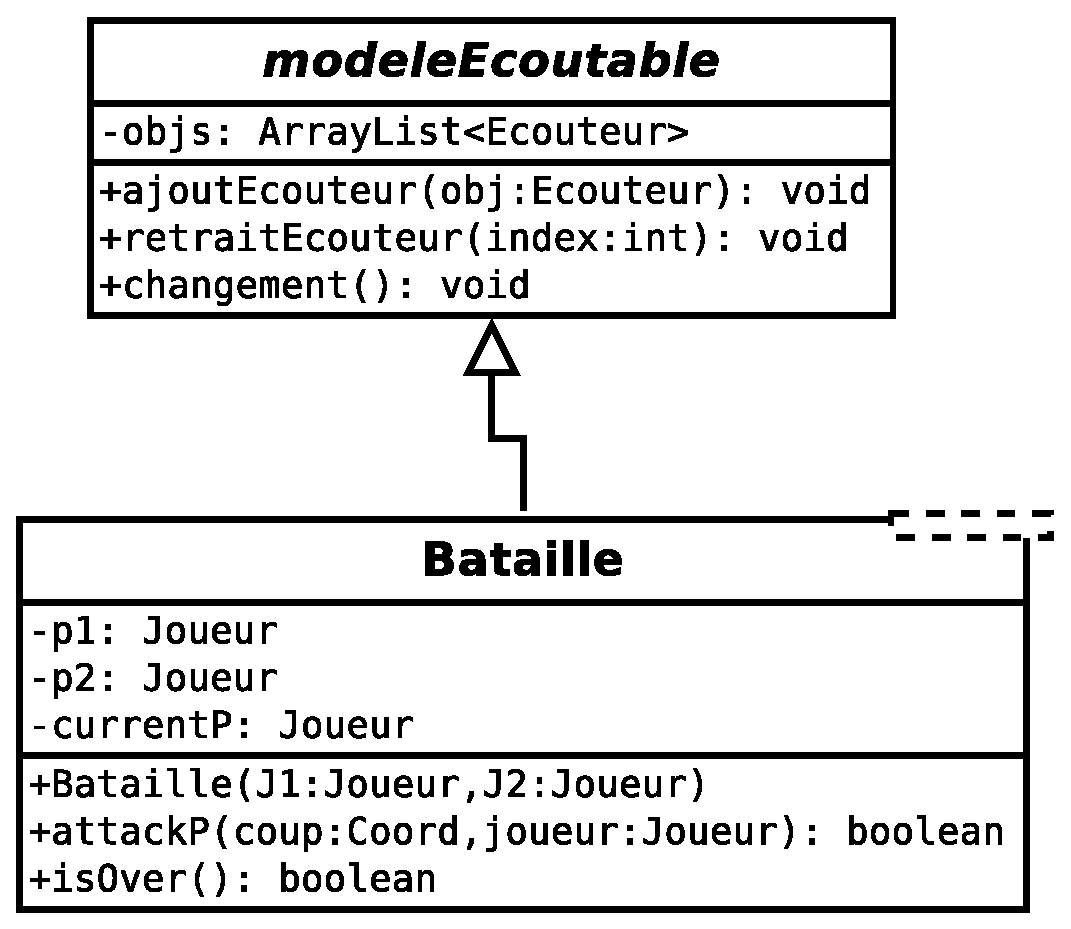
\includegraphics[scale=0.45]{images/Diagramme/package_modele.eps}
\caption{\label{fig:Modele}Package modele}
  
\end{figure}

\begin{figure}[htp]
\centering
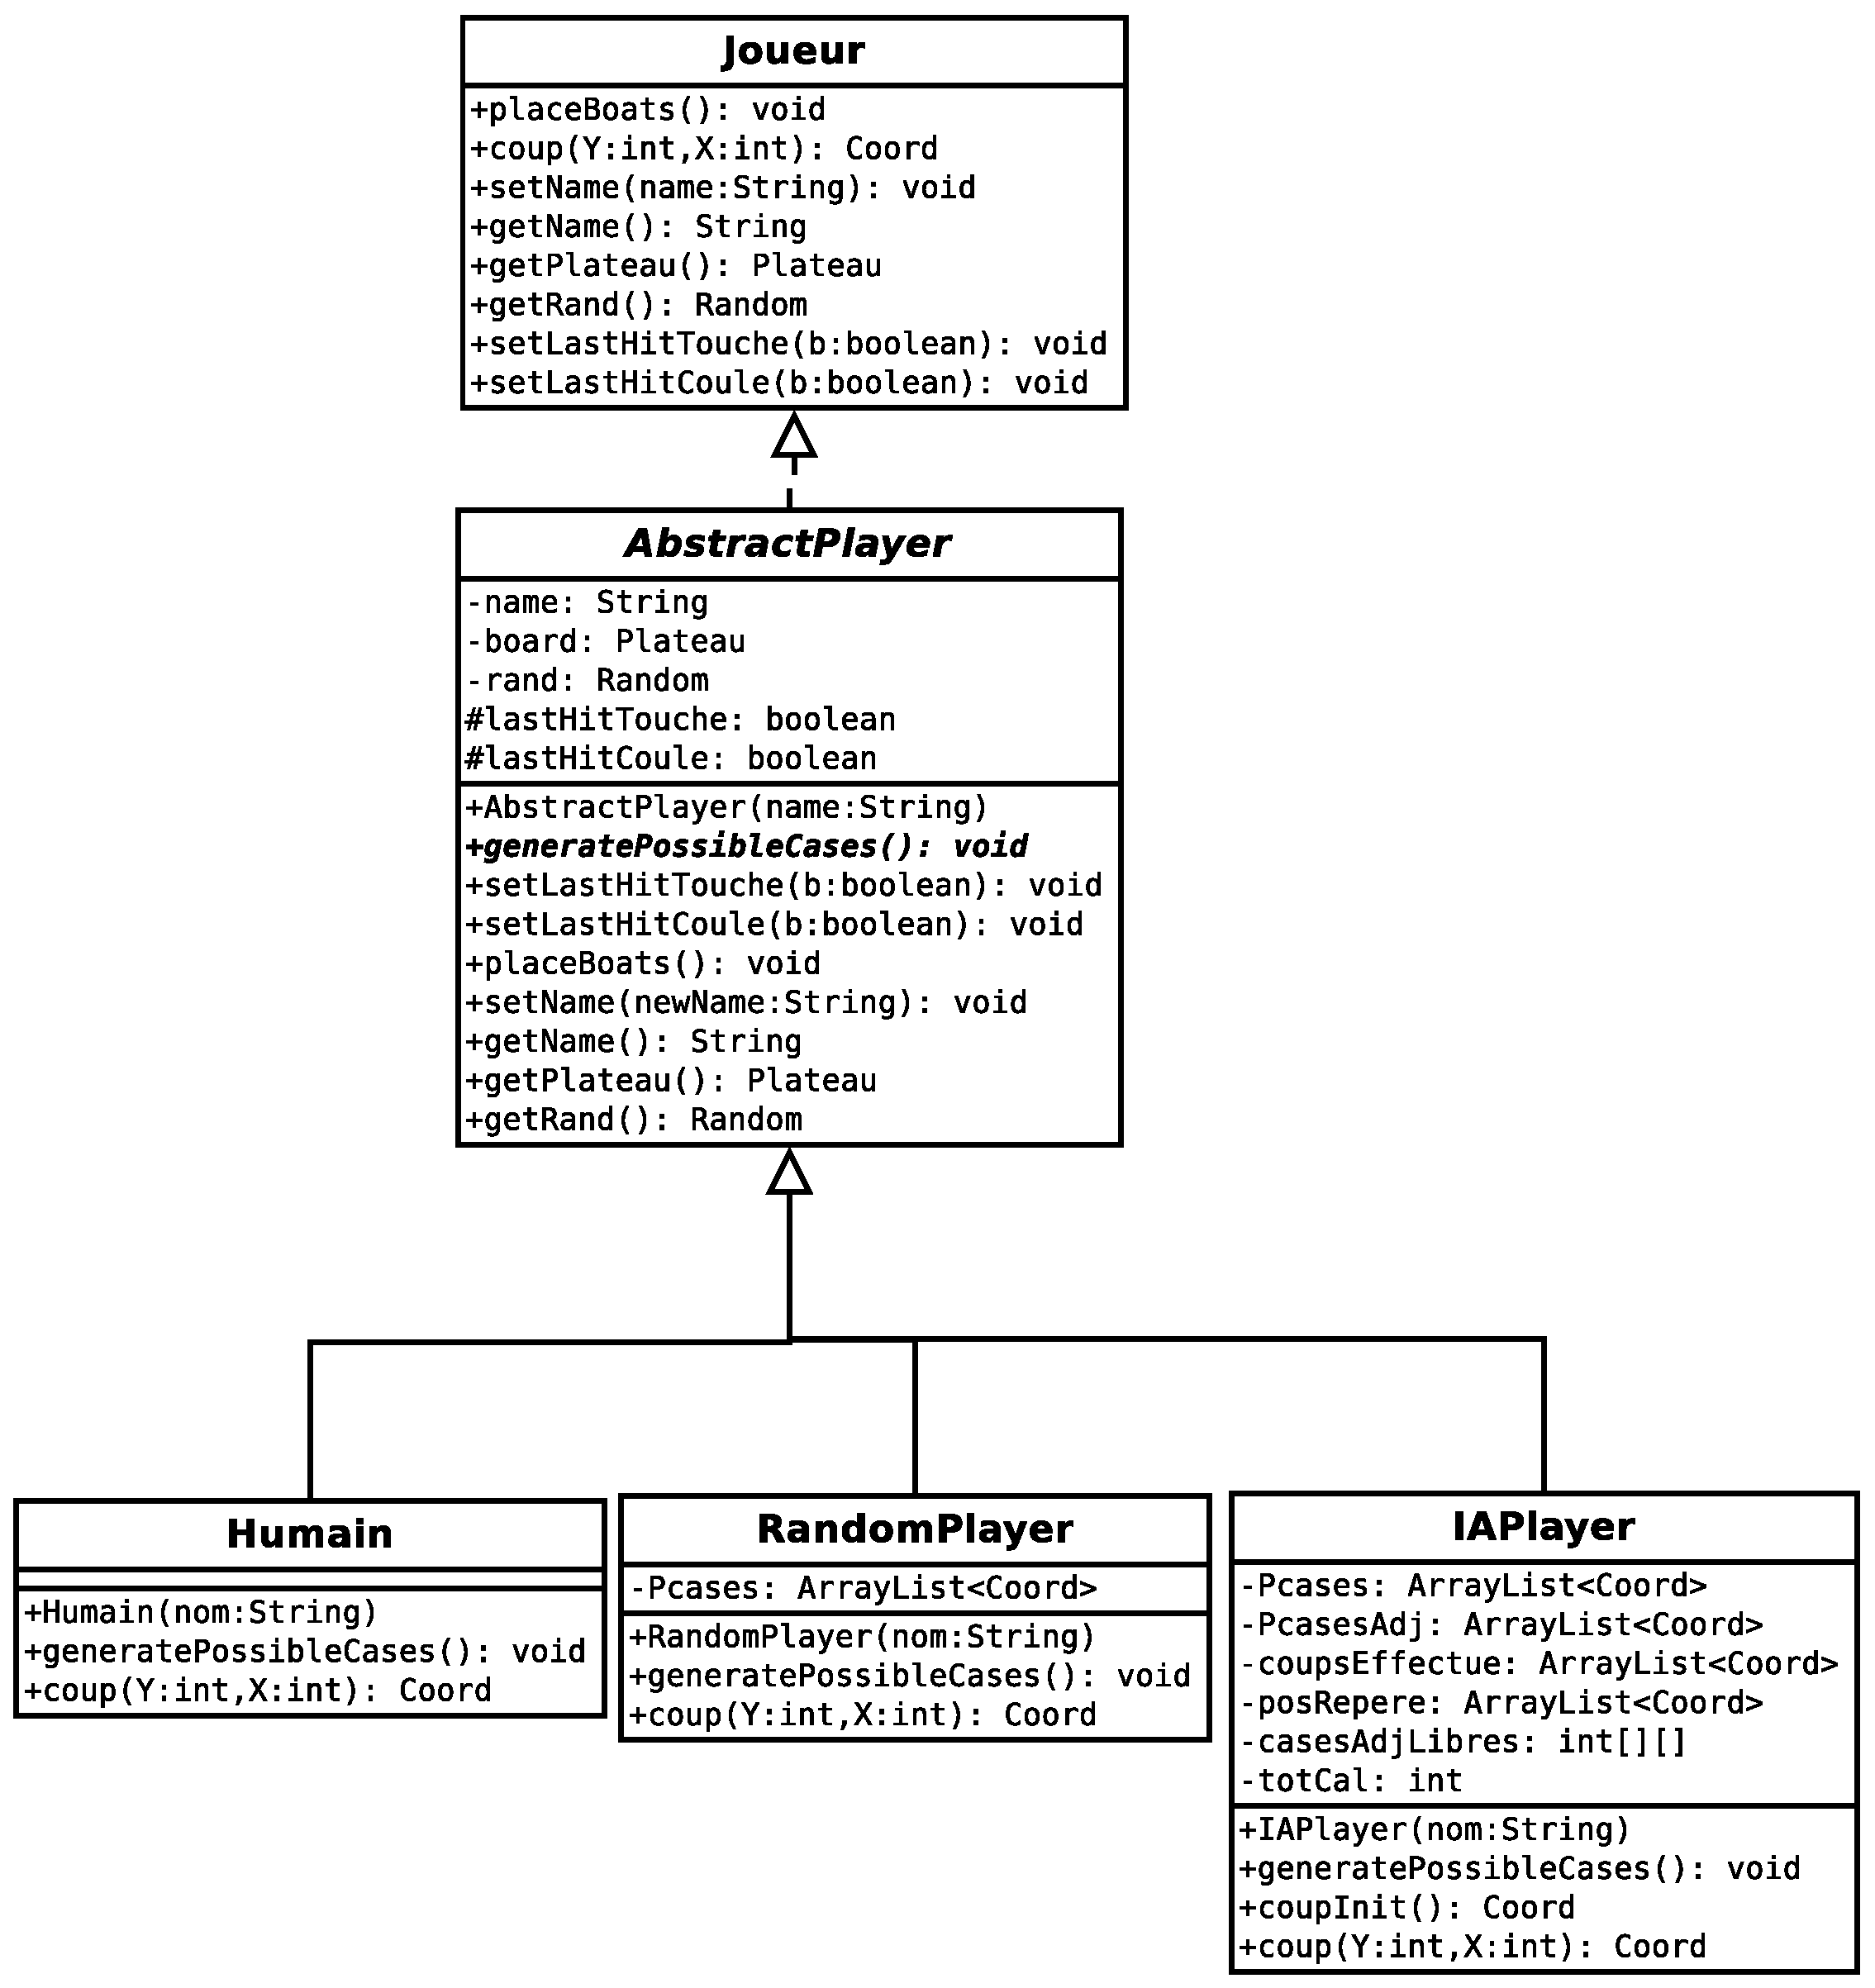
\includegraphics[scale=0.4]{images/Diagramme/package_player.eps}
\caption{\label{fig:Player}Package player}
\end{figure}

\begin{figure}[htp]
\centering
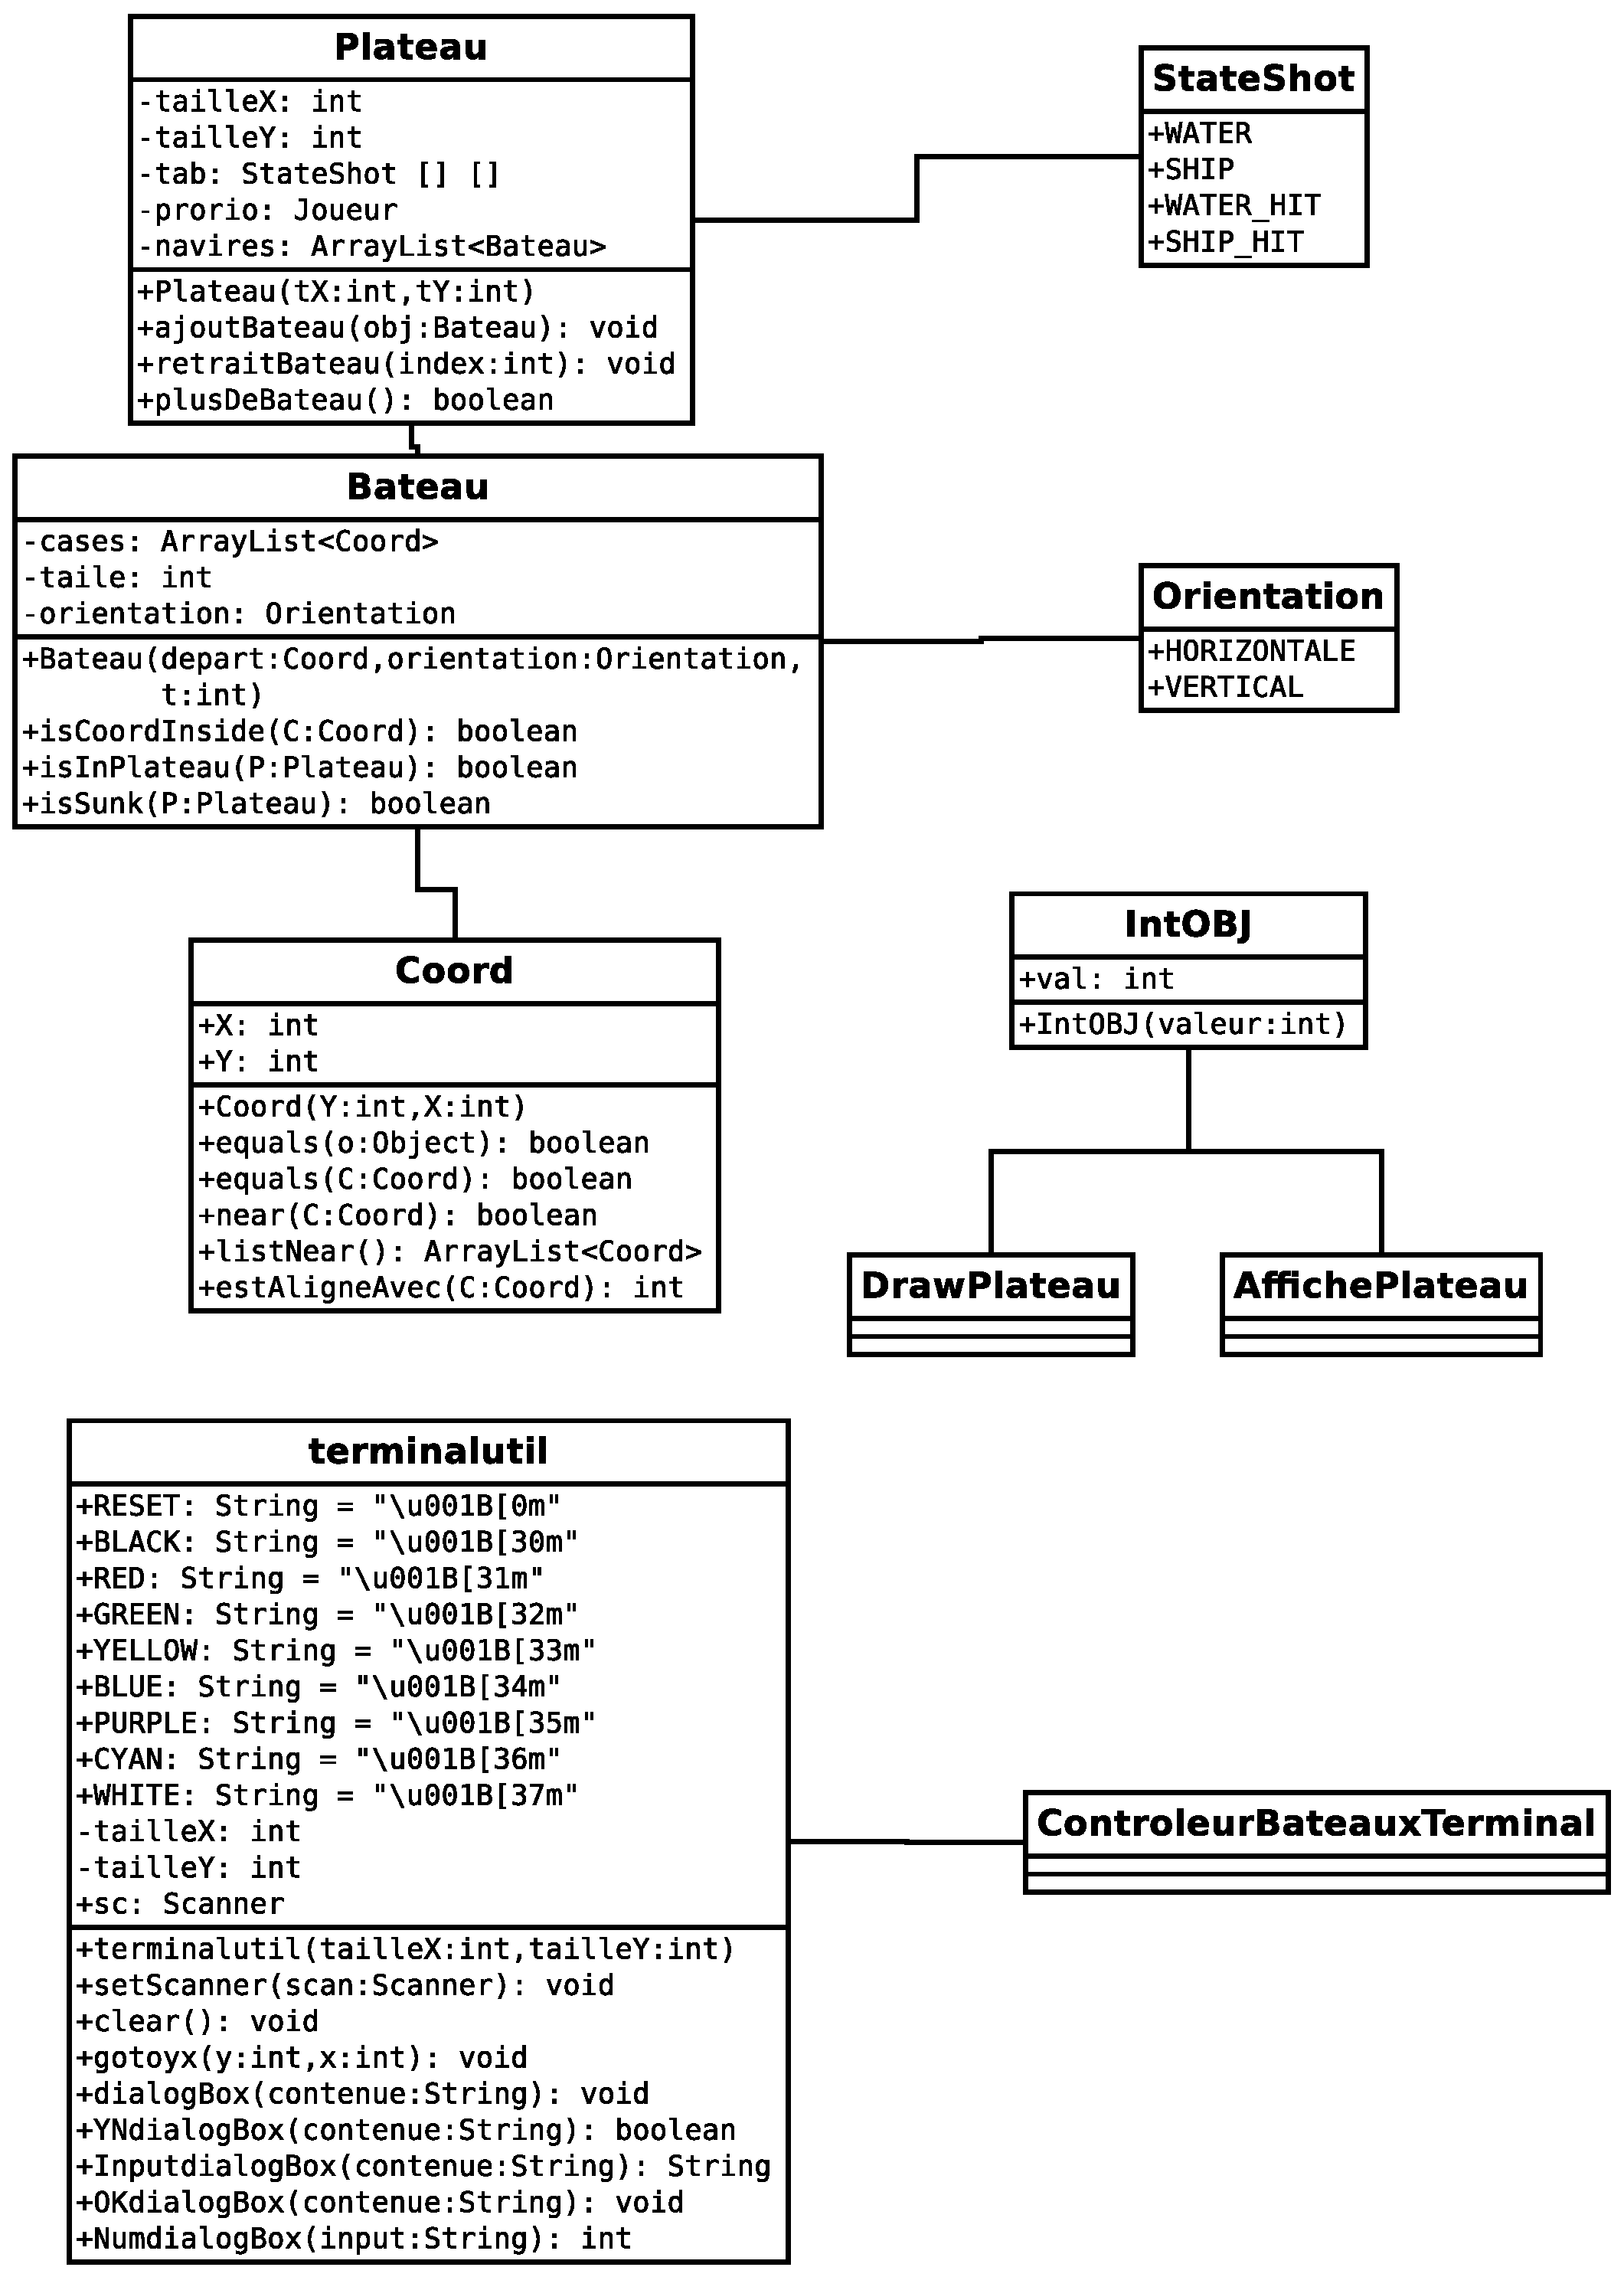
\includegraphics[scale=0.4]{images/Diagramme/package_jeu.eps}
\caption{\label{fig:Jeu}Package jeu}
\end{figure}

\begin{figure}[htp]
\centering
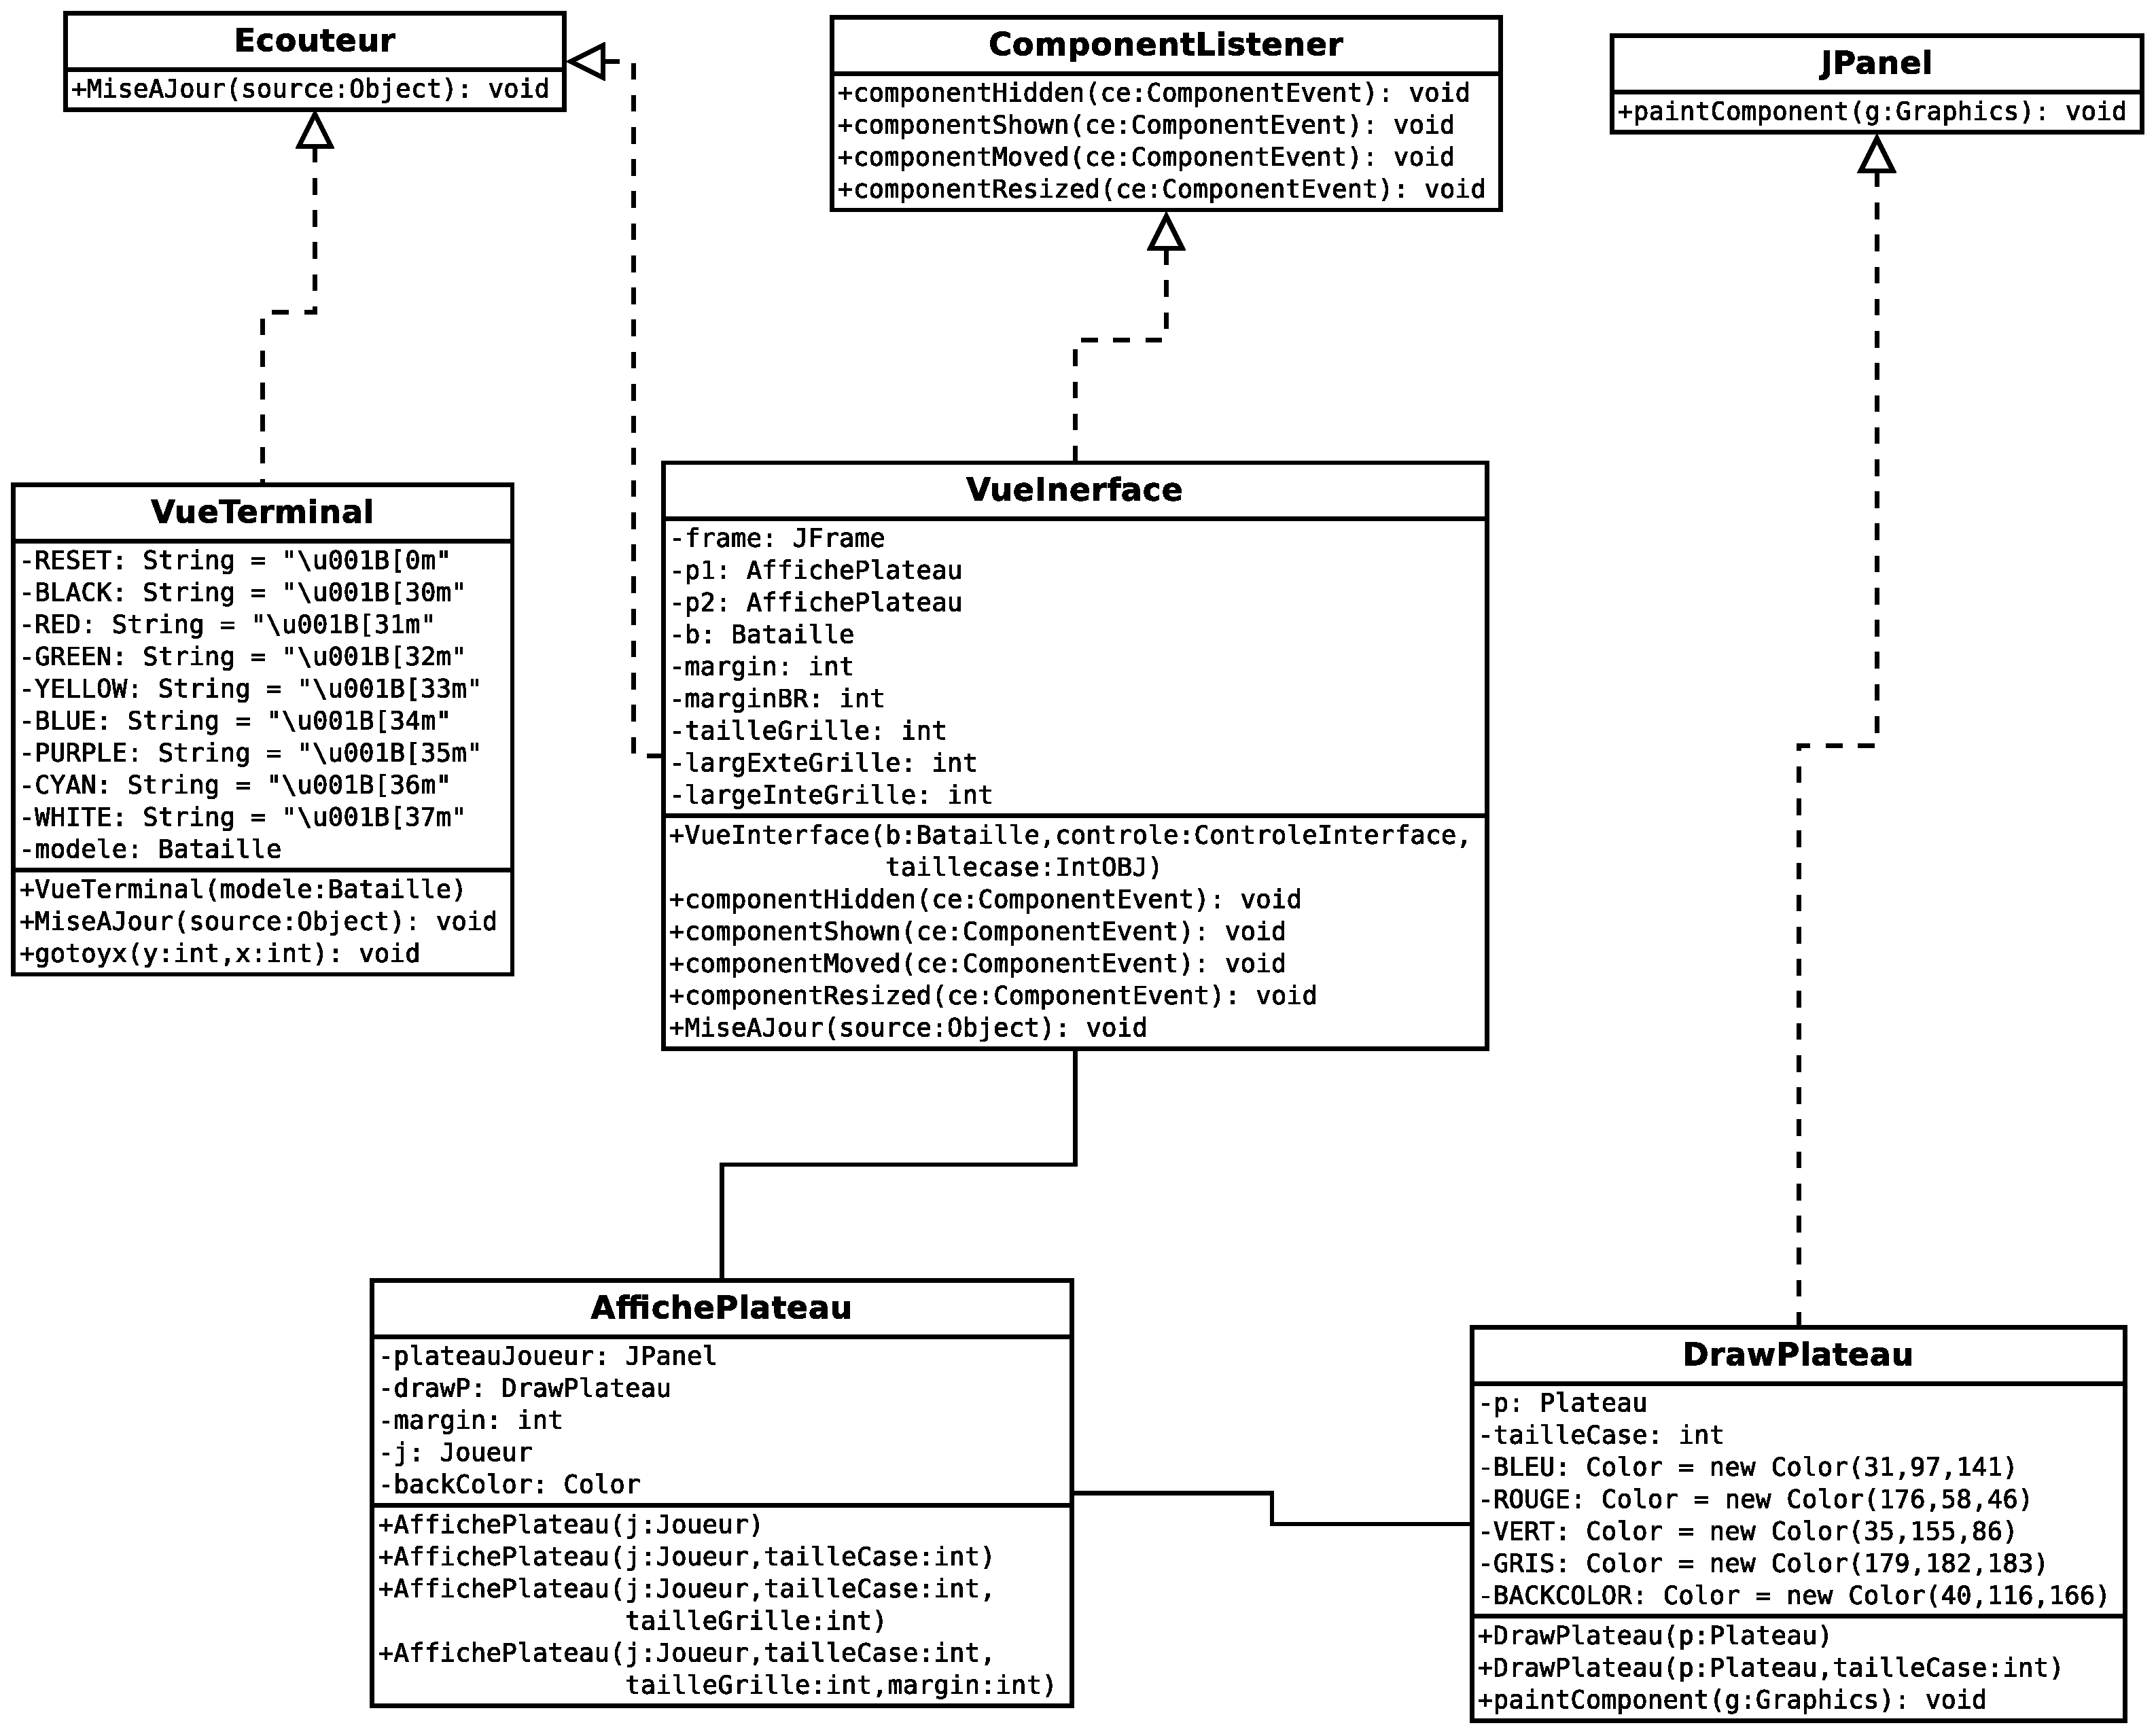
\includegraphics[scale=0.30]{images/Diagramme/package_vue.eps}
\caption{\label{fig:Vue}Package vue}
\end{figure}

\begin{figure}[htp]
\centering
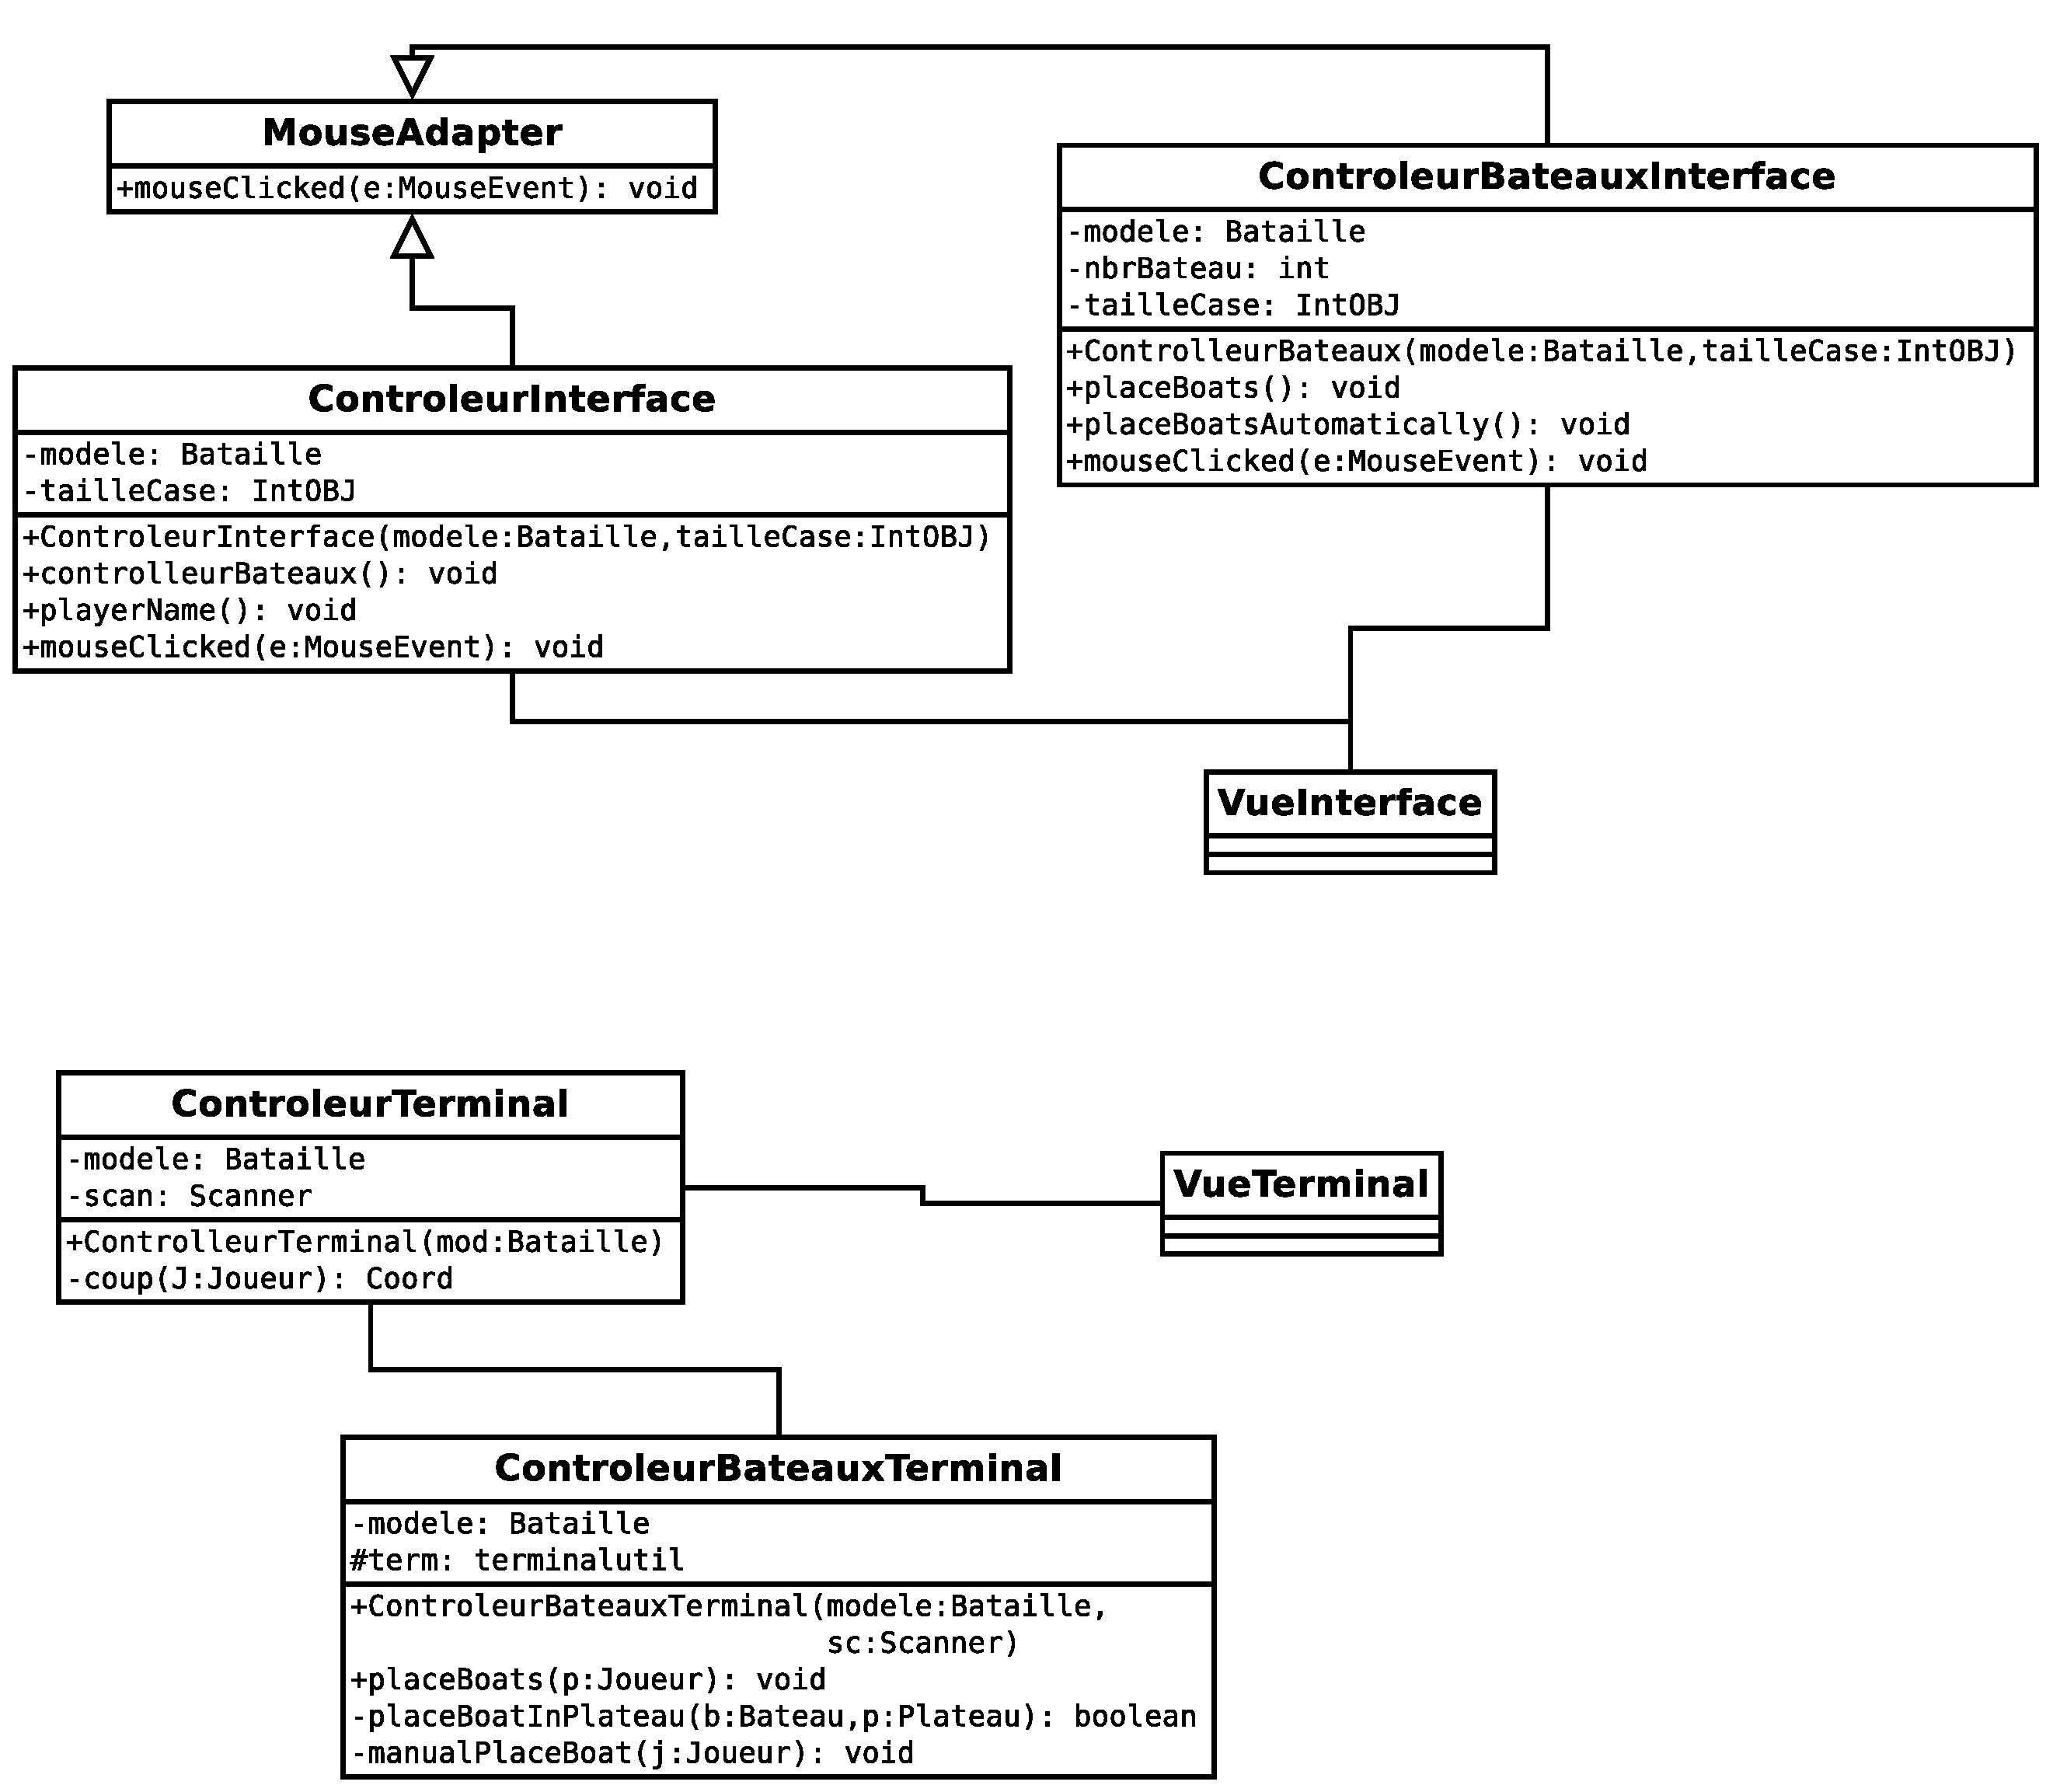
\includegraphics[scale=0.30]{images/Diagramme/package_controleur.eps}
\caption{\label{fig:Controleur}Package controleur}
\end{figure}

\end{document}
